

\tikzset{every picture/.style={line width=0.75pt}} %set default line width to 0.75pt        

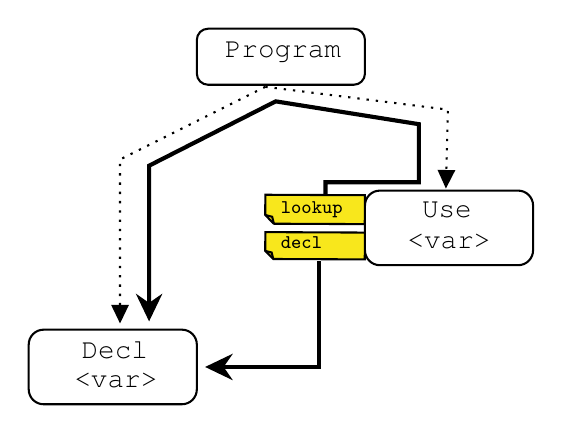
\begin{tikzpicture}[x=0.75pt,y=0.75pt,yscale=-1,xscale=1]
%uncomment if require: \path (0,300); %set diagram left start at 0, and has height of 300

%Rounded Rect [id:dp3127848027298673] 
\draw   (106,28.4) .. controls (106,25.42) and (108.42,23) .. (111.4,23) -- (181.6,23) .. controls (184.58,23) and (187,25.42) .. (187,28.4) -- (187,44.6) .. controls (187,47.58) and (184.58,50) .. (181.6,50) -- (111.4,50) .. controls (108.42,50) and (106,47.58) .. (106,44.6) -- cycle ;
%Rounded Rect [id:dp4023983884044836] 
\draw   (25,175.19) .. controls (25,171.22) and (28.22,168) .. (32.19,168) -- (98.81,168) .. controls (102.78,168) and (106,171.22) .. (106,175.19) -- (106,196.75) .. controls (106,200.72) and (102.78,203.94) .. (98.81,203.94) -- (32.19,203.94) .. controls (28.22,203.94) and (25,200.72) .. (25,196.75) -- cycle ;
%Rounded Rect [id:dp2219004733935539] 
\draw   (187,108.19) .. controls (187,104.22) and (190.22,101) .. (194.19,101) -- (260.81,101) .. controls (264.78,101) and (268,104.22) .. (268,108.19) -- (268,129.75) .. controls (268,133.72) and (264.78,136.94) .. (260.81,136.94) -- (194.19,136.94) .. controls (190.22,136.94) and (187,133.72) .. (187,129.75) -- cycle ;
%Straight Lines [id:da026150514578629602] 
\draw  [dash pattern={on 0.84pt off 2.51pt}]  (139,51) -- (69,86) -- (69,162) ;
\draw [shift={(69,165)}, rotate = 270] [fill={rgb, 255:red, 0; green, 0; blue, 0 }  ][line width=0.08]  [draw opacity=0] (8.93,-4.29) -- (0,0) -- (8.93,4.29) -- cycle    ;
%Straight Lines [id:da14143422944296458] 
\draw  [dash pattern={on 0.84pt off 2.51pt}]  (139,51) -- (227,62) -- (226.08,97) ;
\draw [shift={(226,100)}, rotate = 271.51] [fill={rgb, 255:red, 0; green, 0; blue, 0 }  ][line width=0.08]  [draw opacity=0] (8.93,-4.29) -- (0,0) -- (8.93,4.29) -- cycle    ;
%Shape: Folded Corner [id:dp7308765740333197] 
\draw  [color={rgb, 255:red, 0; green, 0; blue, 0 }  ,draw opacity=1 ][fill={rgb, 255:red, 248; green, 231; blue, 28 }  ,fill opacity=1 ] (138.96,130.05) -- (139,121) -- (186.97,121.22) -- (186.91,134.15) -- (142.82,133.95) -- cycle -- (138.96,130.05) ; \draw  [color={rgb, 255:red, 0; green, 0; blue, 0 }  ,draw opacity=1 ] (142.82,133.95) -- (142.06,130.84) -- (138.96,130.05) ;
%Straight Lines [id:da07267398713805828] 
\draw [color={rgb, 255:red, 0; green, 0; blue, 0 }  ,draw opacity=1 ][line width=1.5]    (165,135) -- (165,185.97) -- (114,185.97) ;
\draw [shift={(110,185.97)}, rotate = 360] [fill={rgb, 255:red, 0; green, 0; blue, 0 }  ,fill opacity=1 ][line width=0.08]  [draw opacity=0] (13.4,-6.43) -- (0,0) -- (13.4,6.44) -- (8.9,0) -- cycle    ;
%Shape: Folded Corner [id:dp2661516004594888] 
\draw  [color={rgb, 255:red, 0; green, 0; blue, 0 }  ,draw opacity=1 ][fill={rgb, 255:red, 248; green, 231; blue, 28 }  ,fill opacity=1 ] (138.96,112.75) -- (139,103) -- (186.98,103.22) -- (186.91,117.15) -- (143.12,116.95) -- cycle -- (138.96,112.75) ; \draw  [color={rgb, 255:red, 0; green, 0; blue, 0 }  ,draw opacity=1 ] (143.12,116.95) -- (142.3,113.6) -- (138.96,112.75) ;
%Straight Lines [id:da38120564451943983] 
\draw [color={rgb, 255:red, 0; green, 0; blue, 0 }  ,draw opacity=1 ][line width=1.5]    (168,103) -- (168,97) -- (213,97) -- (213,69) -- (144,58) -- (83,89) -- (83,160) ;
\draw [shift={(83,164)}, rotate = 270] [fill={rgb, 255:red, 0; green, 0; blue, 0 }  ,fill opacity=1 ][line width=0.08]  [draw opacity=0] (13.4,-6.43) -- (0,0) -- (13.4,6.44) -- (8.9,0) -- cycle    ;

% Text Node
\draw (49,172) node [anchor=north west][inner sep=0.75pt]   [align=left] {{\fontfamily{pcr}\selectfont Decl}};
% Text Node
\draw (45.5,188) node [anchor=north west][inner sep=0.75pt]   [align=left] {{\fontfamily{pcr}\selectfont <var>}};
% Text Node
\draw (213,105) node [anchor=north west][inner sep=0.75pt]   [align=left] {{\fontfamily{pcr}\selectfont Use}};
% Text Node
\draw (206,121) node [anchor=north west][inner sep=0.75pt]   [align=left] {{\fontfamily{pcr}\selectfont <var>}};
% Text Node
\draw (145.01,121.9) node [anchor=north west][inner sep=0.75pt]  [font=\scriptsize] [align=left]  {$\Asyn{\texttt{decl}}$};
% Text Node
\draw (118,28) node [anchor=north west][inner sep=0.75pt]   [align=left] {{\fontfamily{pcr}\selectfont Program}};
% Text Node
\draw (145.01,104.9) node [anchor=north west][inner sep=0.75pt]  [font=\scriptsize] [align=left] {$\Ainh{\texttt{lookup}}$};


\end{tikzpicture}
